%%%%%%%%%%%%%%%%%%%%%%%%%%%%%%%%%%%%%%%%%
% Dreuw & Deselaer's Poster
% LaTeX Template
% Version 1.0 (11/04/13)
%
% Created by:
% Philippe Dreuw and Thomas Deselaers
% http://www-i6.informatik.rwth-aachen.de/~dreuw/latexbeamerposter.php
% 
% This template has been downloaded from:
% http://www.LaTeXTemplates.com
%
% License:
% CC BY-NC-SA 3.0 (http://creativecommons.org/licenses/by-nc-sa/3.0/)
%
%%%%%%%%%%%%%%%%%%%%%%%%%%%%%%%%%%%%%%%%%

%----------------------------------------------------------------------------------------
%	PACKAGES AND OTHER DOCUMENT CONFIGURATIONS
%----------------------------------------------------------------------------------------

\documentclass[final,hyperref={pdfpagelabels=false}]{beamer}

%\setbeamercolor{block title}{fg=black,bg=orange!70} % Change the block title color

%packages
\usepackage{natbib}
\usepackage{amsmath}
\usepackage{amsthm}
\usepackage{mathtools}
\usepackage{mdframed}
\usepackage{subfigure}
\usepackage{booktabs}
% \usepackage{hyperref}
\usepackage{subfigure}
\usepackage{siunitx} % Provides the \SI{}{} and \si{} command for typesetting SI units
\usepackage{graphicx} % Required for the inclusion of images
% \usepackage{natbib} % Required to change bibliography style to APA
\usepackage{datetime}
\usepackage{lscape}
\usepackage{algorithm}
\usepackage{algorithmic}
\usepackage{xspace}
\usepackage[english]{babel} % English language/hyphenation
\usepackage{proof}
\usepackage{booktabs} % Top and bottom rules for tables
\usepackage[colorlinks, allcolors = blue,]{hyperref}
\usepackage{accents}
\usepackage{amsfonts}
\usepackage{stmaryrd}
\usepackage{amsmath,amsthm,amssymb,latexsym} 
\usepackage{microtype}
\usepackage{graphicx}
\usepackage{subfigure}
\usepackage{booktabs} % for professional tables
\usepackage{hyperref}
\usepackage{icml2019}
\usepackage{lipsum}

\usepackage{authblk}


%new commands
\newcommand{\theHalgorithm}{\arabic{algorithm}}
\newtheorem{definition}{Definition}
\usepackage{cancel}
\usepackage[normalem]{ulem}
\newcommand{\dataobs}{\textbf{x}}
\newcommand{\adj}[2]{\textbf{adj}(#1,#2)}
\newcommand{\candidateset}{\mathcal{R}_{\textup{post}}}
\newcommand{\bprior}{\boldsymbol{\beta}_{\textup{prior}}}
\newcommand{\bysinfer}{\mathsf{Infer}}
\newcommand{\betad}{\mathsf{Beta}}
\newcommand{\betaf}{\textup{B}}
\newcommand{\mbetaf}{\boldsymbol{\textup{B}}}
\newcommand{\vtheta}{\boldsymbol{\theta}}
\newcommand{\valpha}{\boldsymbol{\alpha}}
\newcommand{\vbeta}{\boldsymbol{\beta}}
\newcommand{\lapmech}{\mathsf{LSDim}}
\newcommand{\ilapmech}{\mathsf{LSHist}}
\newcommand{\binomial}[2]{\mathsf{Bin}(#1, #2)}
\newcommand{\multinomial}[2]{\mathsf{Mult}(#1, #2)}
\newcommand{\expmech}{\mathsf{EHD}}
\newcommand{\hexpmech}{\mathsf{EHDS}}
\newcommand{\lexpmech}{\mathsf{EHDL}}
\newcommand{\hexpmechd}{\mathsf{expMech}^{D}_{\hellinger}}
\newcommand{\privinfer}{\mathsf{PrivInfer}}
\newcommand{\hlg}{\mathsf{H}}
\newcommand{\dirichlet}[1]{\mathsf{Dir}(#1)}
\newcommand{\alphas}{\boldsymbol{\alpha}}
\newcommand{\xis}{\boldsymbol{\xi}}
\newcommand{\iverson}[1]{[#1]}
\newcommand{\datauni}{\mathcal{X}}
\newcommand{\hellinger}{\mathcal{H}}
\newcommand{\ux}[1]{u(\textbf{x}, {#1})}
\newcommand{\uxadj}[1]{u(\textbf{x}', {#1})}
\newcommand{\cardinality}[2]{\mathcal{C}^{#1}_{#2}}
\newcommand{\range}{\mathcal{O}}
\newcommand{\nomalizer}[1]{\sum\limits_{r'\in \mathcal{R}_{\textup{post}}} \exp \big(\frac{-\epsilon\cdot \mathcal{H} (\mathsf{BI}(#1),r')}{4 \cdot S(#1)}\big)}

\newcommand{\unomalizer}[1]{\sum\limits_{r'\in \mathcal{R}_{\textup{post}}} \exp \big(\frac{-\epsilon\cdot u(#1, r')}{4 \cdot S(#1)}\big)}


\newcommand{\hexpmechPr}[2]{\underset{z \thicksim \hexpmech(#1)}{\Pr}\left[ #2 \right]}
\newcommand{\lapmechPr}[2]{\underset{z \thicksim \lapmech(#1)}{\Pr}\left[ #2 \right]}

\newcommand{\ilapmechPr}[2]{\underset{
{z \thicksim \ilapmech(#1)}
}{\Pr}\left[ #2 \right]}

\newtheorem{thm}{Theorem}[section]

\newtheorem{lem}{Lemma}[section]

\newtheorem{assert}{Assertion}[lem]
\newcommand{\lap}[2]{\mathsf{Lap}(#1, #2)}
\newcommand{\todo}[1]{{\footnotesize \color{red}\textbf{[[ #1 ]]}}}

\usepackage[orientation=landscape,size=custom,width=101.6,height=76.2,scale=1.4]{beamerposter}
%\usepackage[orientation=portrait,size=a0,scale=1.4]{beamerposter} % Use the beamerposter package for laying out the poster with a portrait orientation and an a0 paper size
\usepackage{proof}
%\usetheme{Icy}
\usetheme{I6pd2} % Use the I6pd2 theme supplied with this template

\setbeamercolor{background canvas}{bg=white!20}
% \setbeamercolor{block title}{fg=white,bg=blue!70}
% \setbeamercolor{block body}{fg=black,bg=blue!10}
\usepackage[english]{babel} % English language/hyphenation

\usepackage{amsmath,amsthm,amssymb,latexsym} % For including math equations, theorems, symbols, etc

%\usepackage{times}\usefonttheme{professionalfonts}  % Uncomment to use Times as the main font
%\usefonttheme[onlymath]{serif} % Uncomment to use a Serif font within math environments

\boldmath % Use bold for everything within the math environment

\usepackage{booktabs} % Top and bottom rules for tables

\graphicspath{{figures/}} % Location of the graphics files

\usecaptiontemplate{\small\structure{\insertcaptionname~\insertcaptionnumber: }\insertcaption} % A fix for figure numbering

\usepackage{stmaryrd}

%MACROS
\newcommand{\interp}[2]{\llbracket {#2} \rrbracket_{#1}}
\newcommand{\stmod}[1]{\mathfrak{M}[{#1}]}


%----------------------------------------------------------------------------------------
%	TITLE SECTION 
%----------------------------------------------------------------------------------------

\title{\LARGE Tailoring Differentially Private Bayesian Inference to Distance Between Distributions} % Poster title

\author{Mark Bun$^\dag$,
Gian Pietro Farina$^{*}$,
Marco Gaboardi$^{*}$,
Jiawen Liu$^{*}$
}


\institute{$^{\dag}$Princeton University, $^{*}$University at Buffalo, SUNY} % Institution(s)

%----------------------------------------------------------------------------------------
%	FOOTER TEXT
%----------------------------------------------------------------------------------------

\newcommand{\leftfoot}{Tailoring Differentially Private Bayesian Inference to Distance Between Distributions} % Left footer text

\newcommand{\rightfoot}{mbun@cs.princeton.edu, \{gianpiet,gaboardi,jliu223\}@buffalo.edu} % Right footer text

%----------------------------------------------------------------------------------------

\begin{document}

\addtobeamertemplate{block end}{}{\vspace*{1ex}} % White space under blocks
\begin{frame}[t] % The whole poster is enclosed in one beamer frame

\begin{columns}[t] % The whole poster consists of two major columns, each of which can be subdivided further with another \begin{columns} block - the [t] argument aligns each column's content to the top

\begin{column}{.015\textwidth}\end{column} % Empty spacer column

\begin{column}{.485\textwidth} % The first column

%----------------------------------------------------------------------------------------
%	OBJECTIVES
%----------------------------------------------------------------------------------------

\begin{block}{Objectives}
% \begin{columns} % Subdivide the first main column
% \begin{column}{.69\textwidth}
\begin{enumerate}
\item Design a differentially private Bayesian inference mechanism.
\item Improve accuracy by calibrating noise  to the sensitivity of a
         metric over distributions (e.g. Hellinger distance ($\hellinger$), $f$-divergences, etc\dots).
\end{enumerate}
\end{block}

%----------------------------------------------------------------------------------------
%	INTRODUCTION
%----------------------------------------------------------------------------------------
            
\begin{block}{Bayesian inference ($\bysinfer$), the Beta-Binomial model example:}
% The first subdivided column within the first main column
% \begin{columns} % Subdivide the first main column
% \begin{column}{.54\textwidth} % The first subdivided column within the first main column
%The prior $\betad(\alpha, \beta)$, with hyperparameters $\alpha,\beta\in\mathbb{R}^{+}$ is conjugate to the likelihood function.
\begin{itemize}
  \item  Prior on {\small $\theta: \mathbb{P}_{\theta}= \betad(\alpha, \beta), \alpha,\beta\in\mathbb{R}^{+}$, observed data $\dataobs= (x_1,\dots, x_n)\in\{0,1\}^{n}, n\in\mathbb{N}$.}

  \item  Likelihood function: {\small $\mathbb{L}_{\theta|\dataobs }= \theta^{\Delta \alpha}(1-\theta)^{n - \Delta \alpha}$, where $\Delta \alpha = \displaystyle\sum_{i=1}^{n}x_i$.}

  \item Posterior on {\small $\theta$: $\bysinfer(x)\equiv\mathbb{P}_{\theta|\dataobs}=\betad(\alpha + \Delta \alpha,\beta + n - \Delta \alpha)\propto\mathbb{L}_{\theta|\dataobs }\cdot \mathbb{P}_{\theta}$.}
\end{itemize}
\end{block}
% and with p.d.f:

% \[
%   \Pr(\theta)\equiv \frac{\theta^{\alpha} (1- \theta)^{\beta}}{\betaf(\alpha,\beta)}
% \]
% where $\betaf(\cdot,\cdot)$ is the beta function.
%----------------------------------------------------------------------------------------
%	MATERIALS
%----------------------------------------------------------------------------------------

\begin{block}{Differentially private Bayesian inference and motivations}
\begin{columns} % Subdivide the first main column
\begin{column}{.69\textwidth}
\begin{enumerate}
\item  Baseline approach: 
  \begin{itemize}
  \item Release $\betad(\alpha +  \lfloor\widetilde{\Delta \alpha}\rfloor^n_0,\beta + n - \lfloor\widetilde{\Delta \alpha}\rfloor^n_0)$,
  \item $\widetilde{\Delta \alpha}\sim \lap{\Delta\alpha}{\frac{S}{\epsilon}}$
  \item \todo{$S\propto ||\cdot ||_{1}$}.
  \item Measure accuracy with a metric over distributions, e.g. $\hellinger$.
  \end{itemize}
  {\color{red}{But $S$ grows linearly with the dimension: too noisy when we generalize to Dirichlet-Multinomial ({\small$\dirichlet(\cdot)$}) model}}. 
\item Another approach:
  \begin{itemize}
    \item Calibrate  noise w.r.t \emph{global} sensitivity of $\hellinger$: {\color{red}{but global sensitivity is still too big.}}
    \item Fig. \ref{fig_sensitivity} shows that there is a gap between global and local sensitivity of $\hellinger$.
    \end{itemize}
  \item A better approach:
    \begin{itemize}
      \item \large{Calibrate noise w.r.t. the \emph{smooth} sensitivity of $\hellinger$.}
    \end{itemize}
\end{enumerate}
\end{column}
\begin{column}{.28\textwidth}
\begin{figure}[ht]
\centering
\includegraphics[width=0.9\textwidth]{poster_0.eps}
\caption{\footnotesize{Sensitivity of $\hellinger$. There is a gap between Global and Local sensitivity.}}
\label{fig_sensitivity}
\end{figure}
% \vspace{.1cm}
\end{column}
\end{columns}

\end{block}

%----------------------------------------------------------------------------------------
% OUR APPROACH
%----------------------------------------------------------------------------------------


\begin{block}{Our approach: smoothed Hellinger distance based exponential mechanism}

We define the mechanism $\hexpmech$ which produces an element $r$ in $\betaset$ with probability:
\[
\mathbb{P}_{r \thicksim \hexpmech} =
\frac 
{\exp \Big(\frac{-\epsilon\cdot\hellinger(\bysinfer(\dataobs),r)}{2\cdot S(\dataobs)}\Big)}
{\sum_{r\in\betaset} \exp \Big(\frac{-\epsilon\cdot\hellinger(\bysinfer(\dataobs),r)}{2\cdot S(\dataobs)}\Big)}
\]
where:
\begin{itemize}
 \small{ \item  $\betaset\equiv\{\betad(\alpha',\beta')\mid \alpha'=\alpha+\Delta\alpha, \beta'=\beta+n-\Delta\alpha\}$. With prior distribution $\bprior=\betad(\alpha, \beta)$.}
  \item \small{$-\hellinger(\bysinfer(\dataobs),r)$ denotes the scoring function.}

  \item \small{$S(\dataobs)\equiv \max_{\dataobs' \in \{0,1\}^{n}}\big\{ LS(\dataobs') \cdot e^{-\gamma\cdot d(\dataobs,\dataobs')}\big\}$: smooth sensitivity\cite{nissim2007smooth}}, $d$ is the
    Hamming distance.
   \item \small{$LS(\dataobs')\equiv\max\limits_{y\in \datauni^n:\adj{y}{\dataobs'}, r\in \mathcal{R}}\lvert \hellinger(\bysinfer(y), r) - \hellinger(\bysinfer(\dataobs'), r)\rvert$ is the local sensitivity of $\dataobs',\gamma =   \ln(1 - \frac{\epsilon}{2 \ln (\frac{\delta}{2 (n + 1)})})$}.
 \end{itemize}


\end{block}


\end{column} % End of the first column

\begin{column}{.01\textwidth}\end{column} % Empty spacer column
 
\begin{column}{.485\textwidth} % The second column






  \begin{block}{Preliminary Experimental Results}
    Experiments are on three mechanisms and plotted as follows:
\begin{itemize}
  \item[-] {\textbf{\color{green}{Green}}}: Baseline approach. %adds noise scaled to sensitivity proportional to dimensionality,
  \item[-] {\textbf{\color{red}{Red}}}: Improved baseline approach with sensitivity $1$ in 2 dimensions and $2$ in higher dimensions, since it's equivalent to histogram problem 
  (posteriors of adjacent data sets differ only in two dimensions).
  \item[-] {\textbf{\color{blue}{Blue}}}: $\hexpmech$.
\end{itemize}
% In Fig. \ref{subfig_concrete_prob_2d} and \ref{subfig_concrete_prob_3d} we plot on the x-axis the Hellinger distance from the true posterior and on the y-axis the
% probability of the distributions with that distance under the different mechanisms. In Fig. \ref{subfig_prior} we present the influence of the prior on the accuracy of the three mechanisms,
% by showing the quartiles of the experimental distribution of the Hellinger distance.
\begin{figure}[H]
\begin{center}
\centering
  \subfigure[2 dimensions with data size $600$]{
    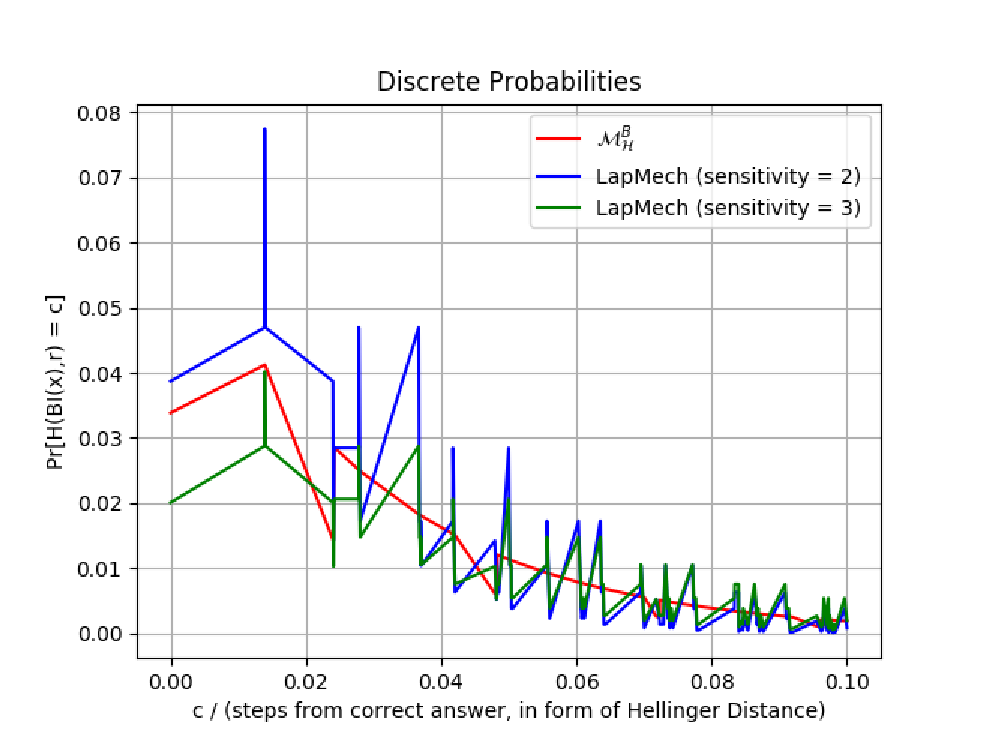
\includegraphics[width=0.31\textwidth]{poster_5.eps}
  \label{subfig_concrete_prob_2d}
  }
  \subfigure[3 dimensions with data size $600$]{
    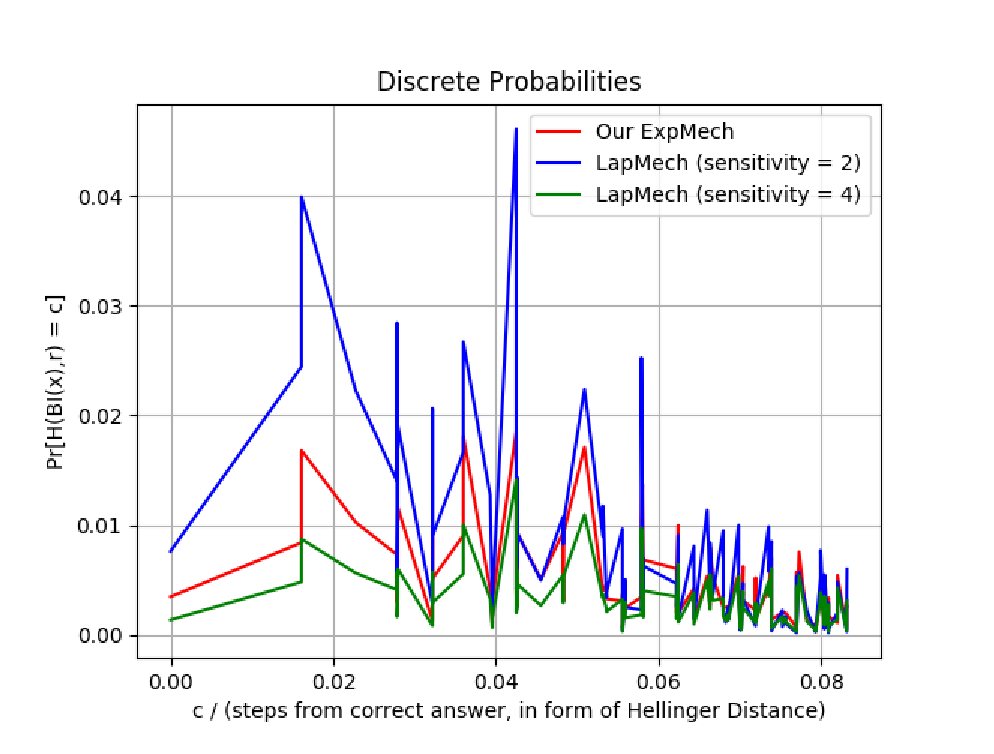
\includegraphics[width=0.31\textwidth]{poster_6.eps}
  \label{subfig_concrete_prob_3d}
  } 
\subfigure[2 dimensions with data size $100$]{
    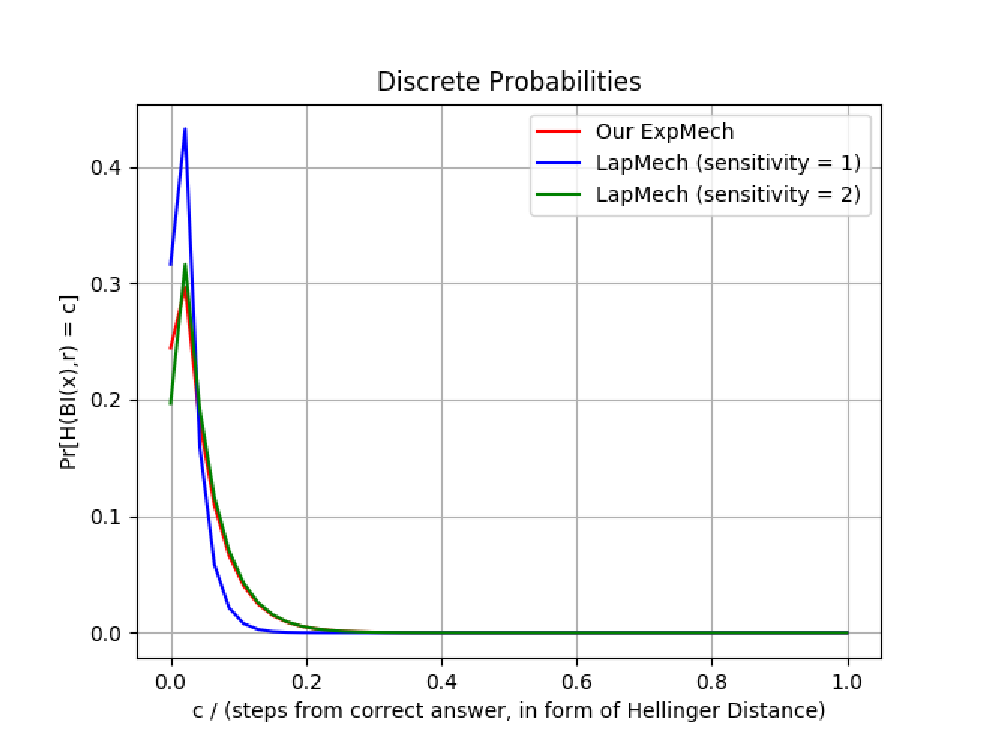
\includegraphics[width=0.313\textwidth]{poster_4.eps}
  \label{subfig_prior}
  }

% \caption{4-quantile and discrete probability plots}
% \label{fig_concrete_prob}
% \end{center}
% \end{figure}
% % Two groups of experimental results both with unit prior $\betad(1,1), \betad(1,1,1)$ and $\betad(1,1,1,1)$, balanced datasets and parameters $\epsilon = 1.0$ and $\delta = 10^{-8}$.
%   Fig. \ref{fig_sampling} and Fig. \ref{subfig_prior} give us the average and 4-quantile of Hellinger distance between the sampled results and true posterior.
% \begin{figure}[H]
% \begin{center}
% \centering
  \subfigure[\footnotesize{2 dimensions, data size $\in [100,500]$}]{
    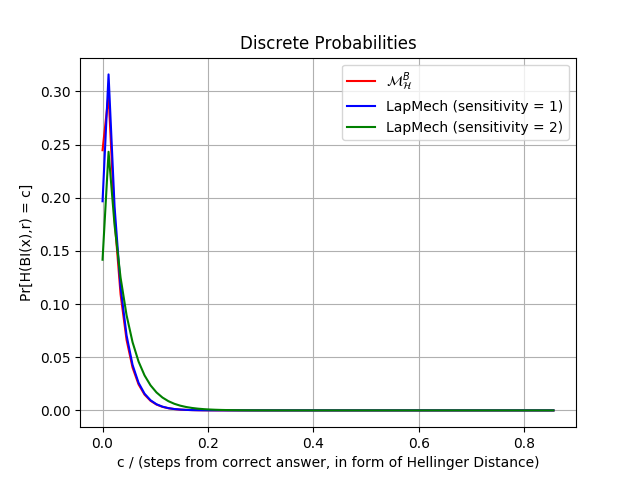
\includegraphics[width=0.333\textwidth]{poster_1.eps}
    \label{subfig_sampling_2d}
  }
  \subfigure[\footnotesize{3 dimensions, data size $\in [100,500]$} ]{
    \includegraphics[width=0.302\textwidth]{poster_2.eps}
  \label{subfig_sampling_3d}
  } 
  \subfigure[\footnotesize{4 dimensions, data size $\in [100,600]$}]{
    \includegraphics[width=0.295\textwidth]{poster_3.eps}
    \label{subfig_sampling_4d}
  }
  \caption{Priors are $\betad(1,1), \dirichlet(1,1,1)$ and $\dirichlet(1,1,1,1)$ (except for Figure \ref{subfig_prior}) ,
    balanced datasets, $\epsilon = 1.0$ and $\delta = 10^{-8}$. }
\label{fig_sampling}
\end{center}


\end{figure}


\end{block}


%----------------------------------------------------------------------------------------
% CONCLUSION
%----------------------------------------------------------------------------------------


\begin{block}{Conclusion}

\begin{itemize}
  \item[-] The smoothed Hellinger distance based exponential mechanism outperforms asymptotically the baseline 
  approach when the latter uses a sensitivity proportional to dimensionality.
  \item[-] Under the same data set size, $\hexpmech$ can outperform LapMech by increasing the prior.
  % \begin{enumerate}
  %   \item  The accuracy that we are going to explore next, and in a more principled and formal way.
    
  %   \item  Experiments have shown that the actual privacy loss
  % in the experiments can be smaller than $\epsilon$. This means that we
  % could improve accuracy, by adding less noise but still achieve
  % $(\epsilon, \delta)$-dp.

  %   \item The choice of the Hellinger distance might seem quite ad-hoc. Hence, it is worth exploring other distances over distributions. An interesting class of probability metrics is the family of $f$-divergences \cite{CIT-004}.

  %   \item Other application of our scheme are going to be explored.
  % \end{enumerate}
\end{itemize}
%\vspace{8mm}
%\vspace{8mm}
%where we require $t$ and $u$ to have distinct sets of free variables.
\end{block}


%----------------------------------------------------------------------------------------
%	RESULTS
%----------------------------------------------------------------------------------------




%------------------------------------------------

% \begin{block}{Results: Figure}

% \begin{figure}
% 
\includegraphics[width=0.8\linewidth]{placeholder.jpg}
% \caption{Figure caption}
% \end{figure}

% \end{block}



%----------------------------------------------------------------------------------------
%	REFERENCES
%----------------------------------------------------------------------------------------

\begin{block}{References}
        
%\nocite{*} % Insert publications even if they are not cited in the poster
\small{\bibliographystyle{unsrt}
\bibliography{bayesian}}

\end{block}

%----------------------------------------------------------------------------------------
%	ACKNOWLEDGEMENTS
%----------------------------------------------------------------------------------------

% \begin{block}{Acknowledgments}

% \begin{itemize}
% \item Nam mollis tristique neque eu luctus. Suspendisse rutrum congue nisi sed convallis. Aenean id neque dolor. Pellentesque habitant morbi tristique senectus et netus et malesuada fames ac turpis egestas.
% \end{itemize}

% \end{block}

%----------------------------------------------------------------------------------------
%	CONTACT INFORMATION
%----------------------------------------------------------------------------------------

\setbeamercolor{block title}{fg=black,bg=white!70} % Change the block title color

% \begin{block}{Contact Information}

% \begin{itemize}
% \item \textbf{Marco Gaboardi}
% \item Web: \href{http://staff.computing.dundee.ac.uk/marcogaboardi/}{http://staff.computing.dundee.ac.uk/marcogaboardi/}
% \item Email: \href{mailto:m.gaboardi@dundee.ac.uk}{m.gaboardi@dundee.ac.uk}
% %\item Phone: +1 617-384-9606
% \end{itemize}

% \end{block}

%----------------------------------------------------------------------------------------

\end{column} % End of the second column

\begin{column}{.01\textwidth}\end{column} % Empty spacer column

\end{columns} % End of all the columns in the poster

\end{frame} % End of the enclosing frame

\end{document}
